\chapter{Contesto applicativo }
\label{contesto}
Nella parte iniziale di questo capitolo viene esplicato il contesto applicativo di questa tesi e, una volta delineato vengono illustrate le tecniche basilari più utilizzate in questo ambito.

\section{Context-aware computing}
\label{context-aware}
Il sistema realizzato nell'ambito di questa tesi, si colloca nel paradigma di computazione noto come \textit{Context-aware computing}, ovvero un'applicazione nel quale i servizi utilizzano informazioni relative al contesto. In \cite{context} si definisce come \textit{context}:

\begin{quotation}
\textit{Ogni informazione che può essere usata per caratterizzare la situazione di un'entità. Ovvero una persona, un posto o un oggetto che è considerato rilevante all'interazione tra l'utente e l'applicazione, inclusi quest'ultimi.}
\end{quotation}

Questa definizione facilita il lavoro di progettazione e sviluppo di un applicazione permettendo di identificare quali informazioni sono importanti e quali no.
Si consideri un'applicazione nel quale l'utente deve registrare il peso degli oggetti presenti nel magazzino tramite una bilancia come mostrato dalla Fig.\ref{fig:context}:

\begin{figure}[H]  
	\centering 
	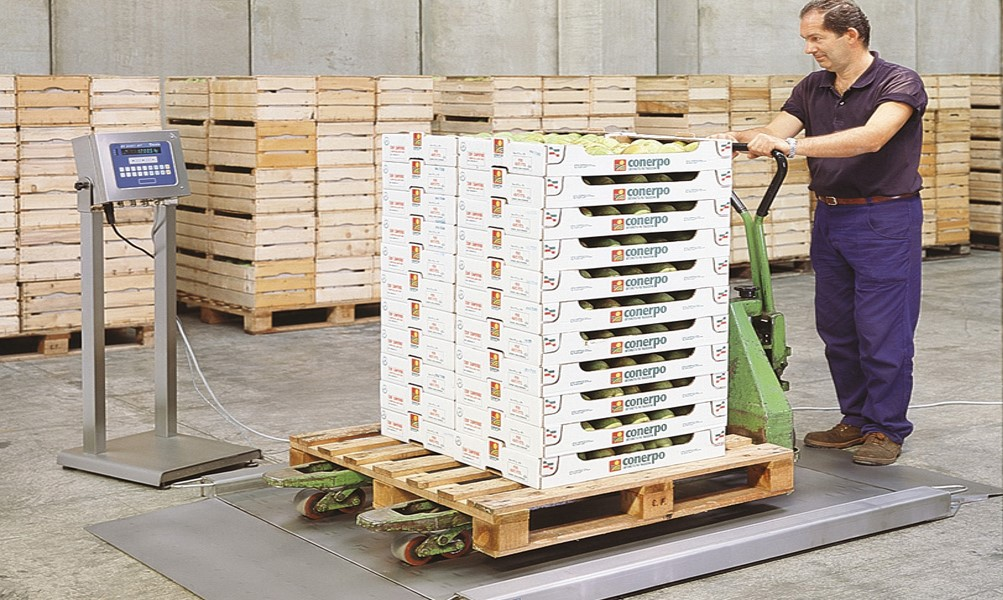
\includegraphics[scale=0.4 ]{ContestoApplicativo/bilancia.jpg}
	\caption{Esempio esplicativo del concetto di contesto}
	\label{fig:context}
\end{figure}
Nello scenario descritto le \textit{entità} sono rispettivamente utente e sistema, mentre due possibili informazioni riguardanti il contesto sono la presenza di altre persone e la posizione geografica del magazzino.\\
La presenza di altre persone nelle vicinanze non influisce sul compito dell'utente, quindi non può essere considerata come informazione contestuale. La posizione geografica del magazzino invece si, infatti se quest'ultimo fosse situato in Italia il peso verrebbe calcolato in chilogrammi mentre se fosse situato negli USA verrebbe calcolato in libbre.\\
I sistemi che reperiscono, usano o interpretano queste informazioni contestuali sono detti \textit{context-aware} e vengono definiti in \cite{context} come:
\begin{quotation}
	\textit{Un sistema è context-aware se usa il contesto per fornire informazioni rilevanti e/o servizi agli utenti, dove la rilevanza dipende dal compito degli utenti.}
\end{quotation}
Uno dei tipi di context-aware più utilizzati si basa sul contesto della localizzazione, ovvero servizi basati sulla conoscenza di dove qualcosa o qualcuno si trovi. Nell'era moderna i servizi basati sulla localizzazione (in inglese: \textit{Location based services} LBSs) stanno assumendo sempre più importanza nelle attività quotidiane dell'uomo grazie alle molteplici possibili applicazioni, tra le quali navigazione assistita per autoveicoli, tracking di persone sensibili (bambini, anziani, malati), servizi di emergenza e così via.\\
I LBSs vengono divisi in due macro categorie:
\begin{itemize}
\label{ops/ips}
	\item \textbf{OPSs}: \textit{Outdoor Positioning System Services}, ovvero servizi di localizzazione in ambienti aperti.
	\item \textbf{IPSs}: \textit{Indoor Positioning System Services}, ovvero servizi di localizzazione in ambienti indoor.
\end{itemize}
La tecnologia satellitare nota come Global Positioning System (GPS) è la tecnologia dominante negli OPSs. Attraverso una rete dedicata di satelliti artificiali in orbita, fornisce ad un terminale mobile o ricevitore GPS informazioni sulle sue coordinate geografiche ed orario, in ogni condizione meteorologica, ovunque sulla Terra o nelle sue immediate vicinanze ove vi sia un contatto privo di ostacoli con almeno quattro satelliti del sistema. La localizzazione avviene tramite la trasmissione di un segnale radio da parte di ciascun satellite e l'elaborazione dei segnali ricevuti da parte del ricevitore \cite{gps}.\\ 
Il grande limite di questa tecnologia è che i ricevitori devono essere nella \textit{line of sight} (letteralmente a vista d'occhio) di almeno quattro satelliti nel cielo, questo significa che all'interno di edifici e spazi chiusi il segnale viene attenuato e i sistemi perdono di accuratezza. Quindi la tecnologia GPS non è adatta ai servizi di localizzazione indoor.\\
Il sistema realizzato nell'ambito di questa tesi si colloca nell'ambito degli IPSs approfonditi nel paragrafo successivo.


\section{Indoor Positioning System Service}
\label{IPS}
Un sistema di posizionamento indoor (in inglese: Indoor positioning system o IPS) è un sistema in grado di localizzare \textit{oggetti} o \textit{persone} all'interno di edifici utilizzando onde radio, campi magnetici, segnali acustici e/o altre informazioni raccolte dai sensori all'interno di dispositivi mobili \cite{IPS} o da altri  appositamente installati nell'ambiente. Questi sono una specializzazione dei più generici sistemi  \textit{Real Time Locating Systems} (RTLS), standardizzati dall'\textit{International
Organization for Standardization and the International Electro Technical Commission} (ISO/IEC 24730). Lo standard definisce i sistemi RTLS come:
\begin{quotation}
	\textit{“ I Real Time Locating System sono sistemi wireless con l'abilità di localizzare la posizione di oggetti ovunque essi siano (in uno spazio definito) con un tempo di risposta che è, o si avvicina, a quello real time. La posizione è derivata dalla misurazione delle proprietà fisiche del collegamento radio."}
\end{quotation}
La differenza tra RTLS e IPS è che gli IPS sono pensati per essere utilizzati da utenti su dispositivi mobili per navigare, orientarsi ed essere tracciati all'interno di edifici, mentre gli RTLS sono più generici e includono anche sistemi di localizzazione real-time che forniscono LBSs di tipo OPSs (Cap.\ref{ops/ips}).\\
Come già accennato, gli IPS \cite{IPS2} permettono di creare una vasta gamma di servizi, ad esempio:
\begin{itemize}
	\item\textbf{Way-Finding}: permettere di navigare in edifici complessi, come ad esempio aeroporti, seguendo il percorso indicato.
	\item\textbf{Ricerca dei punti d'interesse}, aumentare la customer experience facendo trovare all’utente ciò che desidera.
	\item \textbf{Multi-Dot}: visualizzare in una mappa le posizioni degli utenti per tracciare persone potenzialmente in pericolo (bambini, anziani).
	\item \textbf{Marketing di prossimità}: realizzare marketing mirati, inviando annunci sulle ultime offerte.
\end{itemize}
L’elenco di cui sopra rappresenta solo un ridotto sottoinsieme dei potenziali campi applicativi (vedi Fig.\ref{fig:surveyApplication}), per questo motivo negli ultimi anni \cite{indoorThesis} l'interesse nella ricerca e nello sviluppo di sistemi di questo tipo è cresciuto sempre più tra le aziende, che hanno percepito la possibilità di grandi profitti in un mercato non ancora del tutto esplorato.
\begin{figure}[H]  
	\centering 
	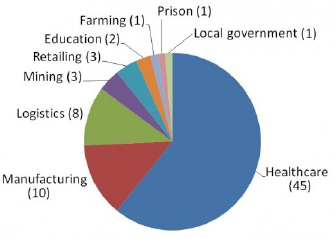
\includegraphics[scale=1.2]{ContestoApplicativo/application.png}
	\caption{Sondaggio tra 74 casi di studio di applicazioni IPS \cite{market}}
	\label{fig:surveyApplication}
\end{figure}

Secondo un sondaggio  di \textit{Markets and Markets} e un articolo pubblicato da\textit{ The International News Magazine}, il mercato degli IPS subirà una crescita annuale media del 42.1\% arrivando a valere 2.60 bilioni di dollari nel 2018. Questo da un'idea del perché grandi aziende come Google, Sony, Microsoft e Apple stiano investendo in questo settore.\\
Un'ulteriore spinta è data dal fatto che, al contrario del GPS per gli OPS (Cap.\ref{context-aware}), tuttora non esiste uno standard di riferimento per gli IPS. Infatti sul mercato sono disponibili diversi tipi di IPS commerciali che si differenziano in base al principio di funzionamento e alle tecniche utilizzate, utilizzando hardware specifico o la combinazione di più sistemi.\\ 




\section{Stima della posizione}
\label{metodi_distanza}
Gli IPS possono essere classificati sulla base di diversi fattori, uno di questi è su come determinano la posizione dei nodi.\\
Stimare \cite{IPS2} la distanza tra dispositivi wireless è utile perché attraverso questa informazione è possibile determinarne (con un certo errore) la posizione di un ricevitore rispetto ad un trasmettitore (\cite{alg1}, \cite{alg2}), queste tecniche si distinguono in:

	\begin{itemize}
	\item \textbf{Range based}:
	
		\begin{itemize}
		\item \textit{RSSI}- potenza del segnale radio ricevuto(sez.\ref{rssi})
		\item \textit{ToA} - tempo d’arrivo: (sez.\ref{toa})
		\item \textit{TDoA} - differenze del tempo di arrivo (sez.\ref{tdoa});
 	    \end{itemize}
     
	\item \textbf{Angle based}:
		\begin{itemize}
			\item \textit{AoA} - Angle of Arrival (sez.\ref{aoa}).
		\end{itemize}
		
\end{itemize}
Per poter determinare le distanze si devono distinguere i punti di riferimento (che hanno
delle coordinate note) dai nodi senza posizione nota a cui assegnare delle coordinate.
Si dicono:
\begin{itemize}
	\item \textbf{Anchor}: i nodi le cui coordinate sono note
	\item \textbf{Target}: il nodo di cui non si conosce la posizione.
\end{itemize}

 L’obiettivo del posizionamento è assegnare le giuste coordinate agli \textit{Unknown} rispetto ad un sistema di riferimento. Questo è strettamente legato all'implementazione dell'IPS e così anche la codifica delle posizioni all'interno del sistema di riferimento, infatti le coordinate potrebbero essere restituite all'utente in maniera relativa ("vicino alla cucina") oppure assoluta ("tre  metri in direzione ovest dal nodo 1").

\subsection{Range based}
Nel posizionamento dei nodi basato sulla distanza la stima della posizione del target dipende dai seguenti parametri:
	\begin{itemize}
	\item il tempo trascorso tra l’emissione e la ricezione del segnale radio;
	\item la distanza euclidea tra ogni emettitore ed il ricevitore;
	\item la potenza del segnale ricevuto.
\end{itemize}
In alcuni casi sono necessarie tre o più \textit{Anchor} per ottenere le coordinate da assegnare allo \textit{Unknown}.

\subsubsection{Received Signal Strength Indicator - RSSI}
\label{rssi}
La comunicazione \cite{IPS2} tra dispositivi wireless (senza fili) avviene tramite lo scambio di segnali propagati nell’aria. Durante la propagazione i segnali tendono ad attenuarsi con l'aumentare della distanza percorsa fino a non essere più percepibili.

\begin{figure}[H]  
	\centering 
	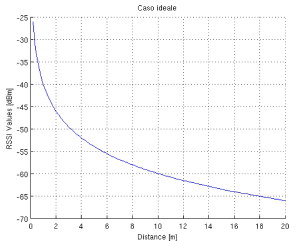
\includegraphics[scale=1.2]{ContestoApplicativo/signal.PNG}
	\caption{RSSI - Andamento della potenza in funzione della distanza percorsa dal segnale}
	\label{fig:signal}
\end{figure}

La stima della potenza del segnale ricevuto è data dall’indicatore RSSI \cite{rssi}. La distanza emettitore-ricevitore si stima utilizzando \textbf{l’equazione di trasmissione di Friis}.

\begin{equation}
		P_{T}=P_{R} \dfrac{G_{T}G_{R}\lambda^2}{(4\pi)^2d^n}
		\label{eq1}
\end{equation}

dove:
\begin{itemize}
	\item $P_{R}$: potenza del segnale ricevuto (Watt)
	\item $P_{T}$: potenza del segnale trasmesso(Watt)
	\item $G_{R}$: guadagno dell'antenna ricevente
	\item $G_{T}$: guadagno dell'antenna trasmittente
	\item $\lambda=\frac{v}{f}$: lunghezza d'onda, dove $v$ è la velocità di propagazione e $f$ è la frequenza dell'onda
	\item $d$: distanza espressa in metri
	\item $n$: constante di propagazione del segnale che dipende dall'ambiente 
\end{itemize}

Con la seguente equazione invece è possibile convertire la potenza espressa in Watt nella potenza espressa in dBm:
\begin{equation}
P[dBm] = 10\log_{10}(10^3P[W])
\label{eq2}
\end{equation}
Combinando l'equazione \ref{eq1} con \ref{eq2} e applicando le proprietà dei logaritmi si ottiene:
\begin{equation}
RSSI = -(10 n \log_{10} d - A)
\label{eq3}
\end{equation}
dove $A$ è la potenza del segnale ricevuto a distanza fissa di un metro (espressa in dBm), considerando una costante di propagazione $n$.\\
La stima della distanza si ottiene infine dalla seguente equazione:
\begin{equation}
d = 10 ^{(\frac{A - RSSI}{10n})}
\label{eq4}
\end{equation}
Tuttavia la distanza restituita non è del tutto precisa, infatti la potenza del segnale potrebbe essere alterata dall'ambiente circostante attraverso i fenomeni di \textbf{Riflessione} (il segnale si riflette su vari ostacoli seguendo più percorsi) e di \textbf{Assorbimento} (il decadimento viene alterato dagli oggetti presenti). Tale tecnica viene solitamente completata utilizzando il metodo della \textbf{Trilaterazione} (sez.\ref{trilaterazione})\\


\subsubsection{Time Of Arrival measurements}  
\label{toa}
A differenza del precedente metodo, con questa tecnica la distanza tra emettitore e ricevitore viene stimata sulla base del tempo impiegato dal segnale a raggiungere il ricevitore. Nello specifico la sequenza di azioni è:
\begin{enumerate}
	\item Il nodo \textit{A} invia il segnale al tempo $t_1$
	\item Il segnale arriva al nodo \textit{B} al tempo $t_2$
	\item \textit{B} elabora il messaggio impiegando un tempo $t_d$ e lo invia al tempo $t_3$
	\item Il segnale torna al nodo \textit{A} al tempo $t_4$
\end{enumerate}
Come mostrato dalla figura seguente:

\begin{figure}[H]  
	\centering 
	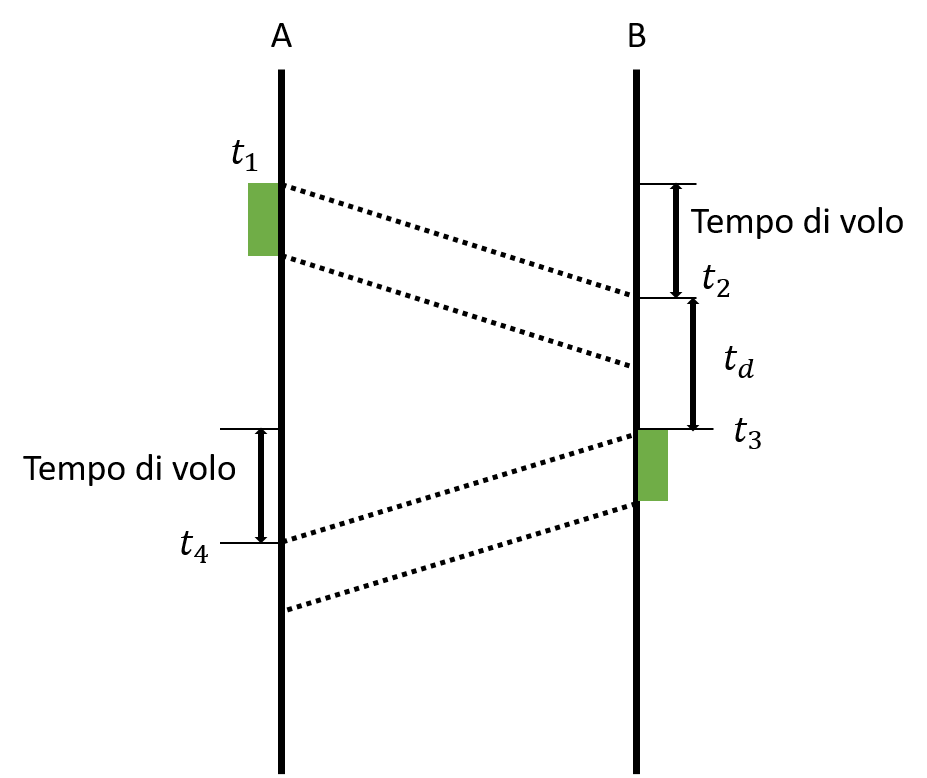
\includegraphics[scale=0.4]{ContestoApplicativo/toa.png}
	\caption{ToA - Principio di funzionamento}
	\label{fig:toa}
\end{figure}

Quindi il tempo di volo può essere ricavato con la seguente equazione:

\begin{equation}
t_d = \dfrac{(t_4 - t_1) - (t_3 - t_2)}{2}
\label{td}
\end{equation}

E infine la distanza stimata attraverso:
\begin{equation}
d_{ToA} = t_d * c
\label{eq:toa}
\end{equation}

dove $c$ è la velocità di propagazione della luce nel vuoto pari a 299792458 m/s. Per identificare in modo univoco un target, questa tecnica viene completata dalla tecnica di posizionamento nota come \textbf{Trilaterazione} (sez. \ref{trilaterazione}), come per le misure RSSI viste precedentemente.\\
Il difetto principale di questa tecnica consiste nel fatto che sistemi utilizzati devono avere un complesso meccanismo di sincronizzazione per mantenere una fonte affidabile di tempo per i sensori\cite{toaProblem}.

\subsubsection{Time Difference Of Arrival}
\label{tdoa}
Questa tecnica è basata sulla differenza nel tempo di arrivo di un segnale emesso da due sorgenti diverse verso un altro nodo, come mostrato in Fig.\ref{fig:tdoa}).

\begin{figure}[H]  
	\centering 
	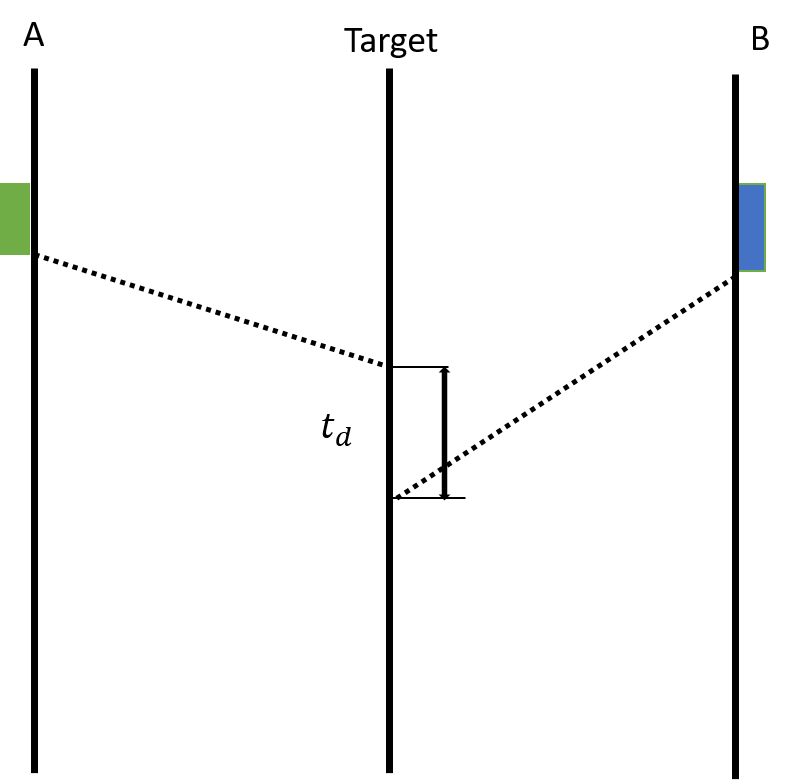
\includegraphics[scale=0.4]{ContestoApplicativo/tdoa.png}
	\caption{TDoA - Principio di funzionamento}
	\label{fig:tdoa}
\end{figure}
Se si suppongono note le posizioni dei nodi \textit{A} e \textit{B} rispetto ad un sistema di riferimento, indicate rispettivamente dalle tuple $(x_B,y_B)$ e $(x_A,y_A)$, la distanza del nodo \textit{Target} può essere stimata dalla seguente equazione:
 
\begin{equation}
\Delta d = \Delta t_d * c
\label{eq:tdoa}
\end{equation}

Dove:
\begin{itemize}
	\item $c$ è la velocità di propagazione della luce nel vuoto
	\item $ \Delta t$ è la differenza del tempo di arrivo dei segnali emessi dai nodi \textit{A} e \textit{B}
	\item $\Delta d$ è la distanza in due dimensioni: $(\sqrt{(x_B-x)^2 + (y_B-y)^2}- \sqrt{(x_A-x)^2 + (y_A-y)^2})$ 
\end{itemize}

In questo modo, la posizione del \textit{target} viene stimata all'interno del luogo geometrico dei punti del piano aventi come costante la differenza delle distanze tra i nodi, ovvero dall'iperbole avente come fuochi i nodi \textit{A} e \textit{B}. Come mostrato in Fig.

\begin{figure}[H]  
	\centering 
	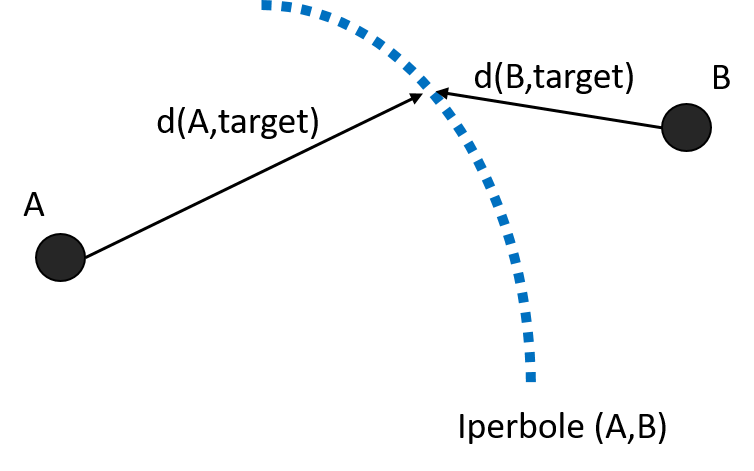
\includegraphics[scale=0.4]{ContestoApplicativo/tdoa1.png}
	\caption{TDoA - Stima della posizione lungo l'iperbole identificata da due nodi}
	\label{fig:tdoa1}
\end{figure}

	Tuttavia così facendo la posizione del \textit{target} rimane stimata in un'insieme di punti infinito, quindi come per le tecniche viste precedentemente (sez.\ref{rssi} e sez.\ref{toa}) per identificare in modo univoco il target questa tecnica ha bisogno di essere completata dalla tecnica di posizionamento nota come \textbf{Trilaterazione} (sez.\ref{trilaterazione}).

\subsection{Angle Based}
\label{angle}
\subsubsection{Angle of Arrival}
\label{aoa}
Con questa tecnica la posizione del \textit{target} viene stimata misurando gli angoli di incidenza del segnale trasmesso ad altri nodi.\\
Si consideri \cite{aoa} un'antenna in un canale di propagazione, la tensione del segnale ricevuto (\ref{fig:aoa}) è data dalla seguente equazione:\\
\begin{equation}
 V = \int_{0}^{2\pi} AoA(\varphi) G(\varphi)d\varphi 
\end{equation}

Dove:
\begin{itemize}
	\item $AoA(\varphi)$ rappresenta l'ampiezza e la fase dell'onda incidente
	\item $G(\varphi)$ è il campo elettrico del nodo target 
	\item $C$ valore proporzionale costante
\end{itemize}

Se si ruota l'antenna di un angolo $\alpha$ intorno a se stessa nel piano cartesiano la precedente equazione diventa:
\begin{equation}
\label{eq:2}
V (\alpha) = \int_{0}^{2\pi} AoA(\alpha-\varphi) G(\varphi)d\varphi 
\end{equation}

Possiamo notare che l'Eq.\ref{eq:2} è la convoluzione di $AoA$ e $G$ e può essere scritta nel seguente modo:
\begin{equation}
\label{eq:3}
V (\alpha) = C AoA(\alpha) * G(\alpha)
\end{equation}

Si è scelto di normalizzare l'Eq.\ref{eq:3} con il valore constante $C$. Quindi, utilizzando la transformata di Fourier l'Eq.\ref{eq:3} diventa:

\begin{equation}
\label{eq:4}
F(V(\alpha)) = F(AoA(\alpha)) F(G(\alpha))
\end{equation}

Da cui è possibile calcolare l'angolo di incidenza desiderato:

\begin{equation}
\label{eq:5}
AoA(\alpha) = F^{-1} \dfrac{F(V(\alpha))}{F(G(\alpha))} \quad se \quad F(G(\alpha))\neq 0
\end{equation}

\begin{figure}[H]  
	\centering 
	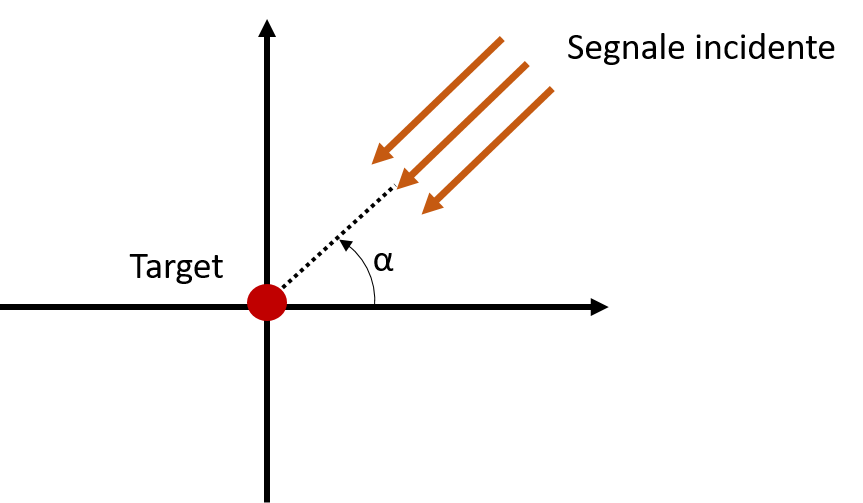
\includegraphics[scale=0.4]{ContestoApplicativo/aoa.png}
	\caption{AoA - Stima della posizione attraverso l'angolo di incidenza}
	\label{fig:aoa}
\end{figure}

Il vantaggio dell’AoA risiede nella possibilità di ottenere un risultato attendibile senza la necessità di informazioni riguardanti i tempi di trasmissione. A fronte del risparmio dal punto di vista computazionale, la tecnica presenta alcuni svantaggi pratici, dovuti al costo dell’hardware, che al fine di restituire informazioni precise, deve essere di alta qualità; rischiando altrimenti di incorrere in fenomeni che comprometterebbero la misurazione. Per questo motivo solitamente questa tecnica viene completata dalla tecnica di posizionamento nota come \textit{Triangolazione} (sez.\ref{triangolazione}).


\section{Tecniche di localizzazione}
Per tecniche di localizzazione si intendono tutte quelle tecniche che, combinate alle differenti metodologie di stima della posizione viste precedentemente (vedi \ref{metodi_distanza}), permettono di localizzare un nodo \textit{target} all'interno di un sistema di riferimento.\\
In questo paragrafo vengono illustrate quelle più conosciute e basilari nell'ambito degli IPS.

\subsection{MIN-MAX}
Combina le stime della distanza di più \textit{anchor}, ottenute attraverso tecnica \textit{RSSI} (sez.\ref{rssi}), nel seguente modo:

\begin{itemize}
	\item Stimare la distanza $d_i$ di ogni nodo i-esimo in base al valore RSSI
	\item Traccia due linee orizzontali e verticali a distanza $d_i$ dal nodo \textit{target}
	\item Identifica un quadrato di lato 2  $d_i$ i cui estremi saranno: \\
			$[max(x_i-d:i),max(y_i-d_i)] * [min(x_i+d_i),min(y_i+d_i))]$
	\item Calcola le intersezioni dei quadrati
\end{itemize}

Il centro del quadrato (Fig.\ref{fig:minmax}) rappresenta la posizione stimata del \textit{target}. Più piccola sarà l’area e maggiore sarà l’accuratezza della posizione stimata.
\begin{figure}[H]  
	\centering 
	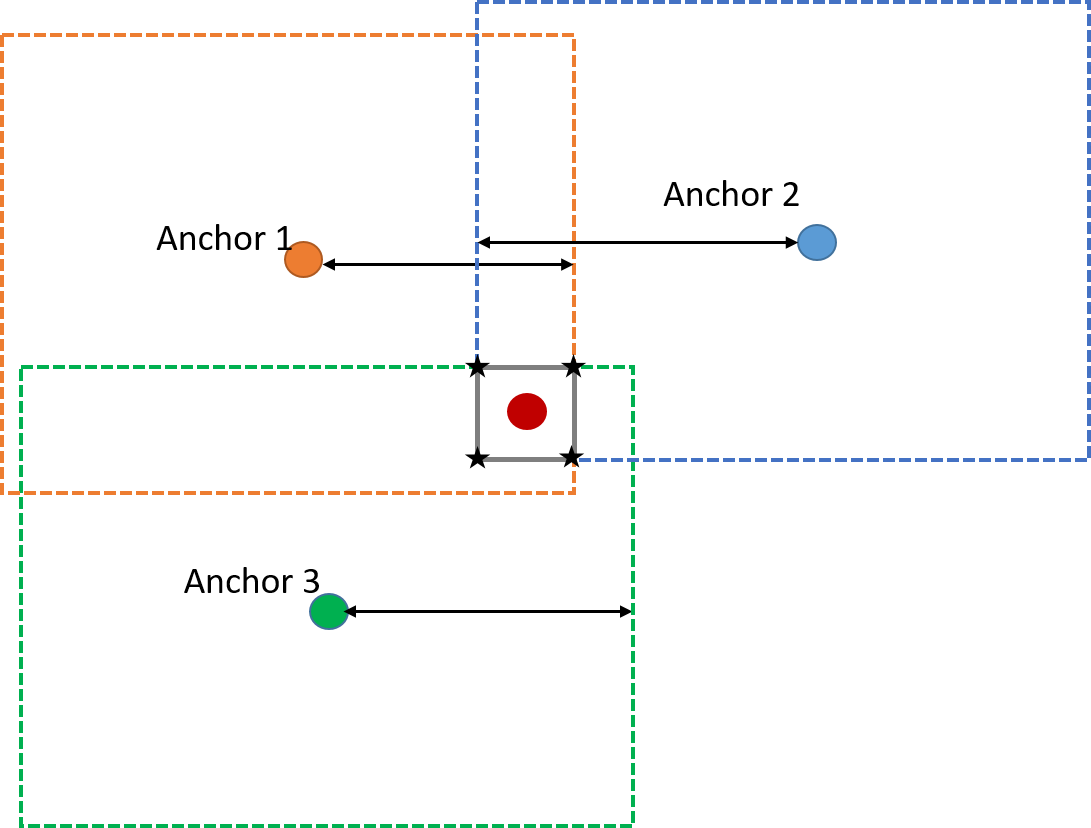
\includegraphics[scale=0.4]{ContestoApplicativo/minmax.png}
	\caption{MIN-MAX - Tecnica di posizionamento }
	\label{fig:minmax}
\end{figure}



\subsection{Trilaterazione}
\label{trilaterazione}
Consideriamo 3 \textit{Anchor} intorno alle quali si disegnano 3 circonferenze aventi per centro le coordinate degli \textit{Anchor} e per raggio l'RSSI del segnale ricevuto dallo \textit{Uknown}, come mostrato in figura:
\begin{figure}[H]  
	\centering 
	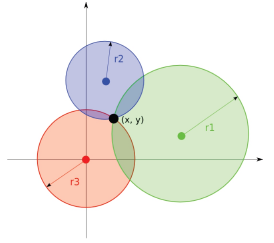
\includegraphics[scale=0.8]{ContestoApplicativo/trilaterazione.png}
	\caption{Trilaterazione - Esempio esplicativo}
	\label{fig:trilaterazione}
\end{figure}
Quindi le coordinate dell'\textit{Unknown} sono la soluzione del seguente sistema:
\begin{equation}
\begin{cases}
(x-x_1)^2 + (y-y_1)^2 = r_1^2\\
(x-x_2)^2 + (y-y_2)^2 = r_2^2\\
(x-x_3)^2 + (y-y_3)^2 = r_3^2
\end{cases}
\end{equation}
In base alla soluzione del sistema si può avere una delle seguenti situazioni:
\begin{itemize}
	\item La soluzione non è unica, si hanno tre cerchi che si sovrappongono
	\item Il sistema non ammette soluzione, i raggi vanno aumentati
	\item La soluzione esiste ed è unica, i tre cerchi si intersecano in un solo punto
\end{itemize}



\subsection{Triangolazione}
\label{triangolazione}
A differenza delle Trilaterazione (sez.\ref{trilaterazione}), queste tecniche identificano la posizione del nodo \textit{target} a partire dagli angoli stimati da tre \textit{anchors} attraverso una delle teniche Angle Based (sez.\ref{angle}).\\
In \cite{triangolazione} si descrive la triangolazione geometrica attraverso il seguente algoritmo:\\

\begin{enumerate}
   \item Siano \textit{1, 2, 3} le \textit{anchor} in grado di stimare l'angolo, rispetto ad una circonferenza concentrica all'\textit{anchor} stessa, del nodo target
   \item siano $L_{12}$ e $L_{31}$ rispettivamente le distanze tra l'\textit{anchor} 1 e 2 e l'\textit{anchor} 3 e 1
   \item Siano gli angoli compresi tra \textit{1} e \textit{2} e tra \textit{1} e \textit{3}, indicati rispettivamente con $\lambda_{12} e \lambda_{13}$, minori di 180°
   \item sia $\phi$ l'angolo tra l'asse x positivo e la linea formata dall'\textit{anchor} \textit{1} e \textit{2}
   \item sia $\sigma$ l'angoolo tra l'asse x positivo, l'\textit{anchor} \textit{1} e l'\textit{anchor} \textit{3} più $\phi$
   \item sia $\gamma= \sigma - \lambda_{31}$
   \item sia $p= \dfrac{L_{31} \sin\lambda_{12}}{L_{12} \sin\lambda_{31}}$
   \item sia $\tau= \tan^{-1} \dfrac{\sin\lambda{12}-p \sin\gamma}{p \cos\gamma-\cos\lambda{12}}$
   \item sia $L_1 = \dfrac{L_{12} sin(\tau+\lambda_{12})}{\sin\lambda_{12}}$
\end{enumerate}

Allora le coordinate $x$ e $y$ del target sono date da:
\begin{itemize}
	\item $x_R = x_1 - L_1  \cos(\phi + \tau)$
	\item $y_R = y_1 - L_1  \sin(\phi + \tau)$
	\item $\Phi_R = \phi + \tau - \lambda_1$
\end{itemize}
Dove $\Phi_R$ rappresenta l'orientamento del nodo target, come mostrato in figura:


\begin{figure}[H]  
	\centering 
	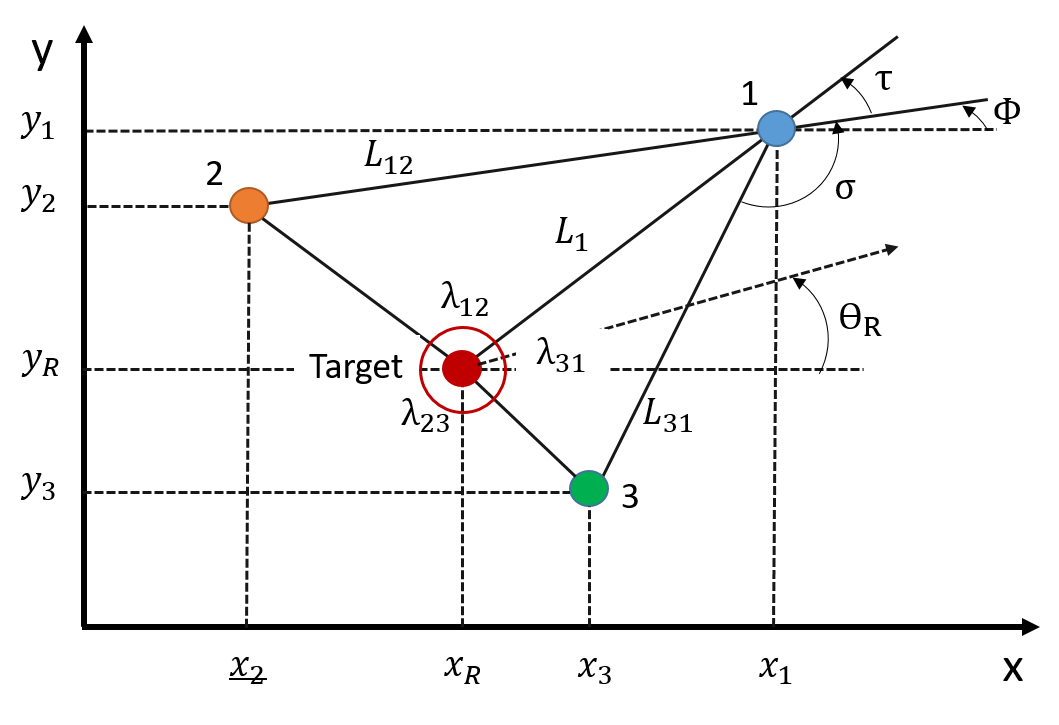
\includegraphics[scale=0.4]{ContestoApplicativo/triangolazione.png}
	\caption{Triangolazione - Esempio esplicativo}
	\label{fig:triangolazione}
\end{figure}





\section{Sensor Data Fusion}

In generale con Sensor Data Fusion si indicano tutte quelle tecniche che \cite{sensorfusion} combinano dati provenienti da sensori o derivate da altre risorse tali che l'informazione risultante abbia una minore incertezza rispetto a quella ottenuta utilizzando le risorse individualmente. \\
Nel contesto degli IPS (\ref{IPS}), il Sensor Fusion ha come scopo quello di determinare informazioni riguardanti la posizione di oggetti e/o persone. Le risorse delle informazioni grezze sono le più svariate, tra le quali:
\begin{itemize}
	\item Accelerometro
	\item Giroscopio
	\item Magnetometro
	\item Infrarossi
	\item RFID 
	\item Sensori ottici
	\item Sensori di pressione
	\item Bluetooth
	\item WiFi
	\item Telecamera
	\item UWB
\end{itemize}

Come e quali risorse utilizzare per stimare la posizione di un oggetto è una sfida ingegneristica non banale, ma grazie alla crescente richiesta di IPSs la ricerca di nuove tecnologie e algoritmi in questo settore ha permesso di raggiungere risultati incredibili. \\







